\documentclass[11pt,a4paper]{scrartcl}
\usepackage[utf8]{inputenc}
\usepackage{amsmath}
\usepackage{amsfonts}
\usepackage{amssymb}
\usepackage{graphicx}
\usepackage{geometry}
\usepackage{tabularx}
\usepackage{array}
\usepackage[section]{placeins}
\usepackage{multicol}
\usepackage[table,xcdraw]{xcolor}
\usepackage{longtable}
\usepackage{rotating}
\usepackage{booktabs}
\usepackage{subcaption}
\geometry{a4paper, top=18mm, left=18mm, right=18mm, bottom=18mm, includefoot}
\definecolor{maroon}{rgb}{0.62, 0.15, 0.20}
\definecolor{timberwolf}{rgb}{0.86, 0.84, 0.82}
\definecolor{navy}{rgb}{0.05, 0.27, 0.44}

\renewcommand{\thesection}{\Alph{section}}

\begin{document}
	\title{The political economy of EU asylum policies}
	\subtitle{ONLINE APPENDIX}
	\author{Martina Burmann, Marcus Drometer and Romuald Méango}
	\maketitle

\tableofcontents

\clearpage
\FloatBarrier
\section{Data Appendix}

\clearpage
\FloatBarrier
\section{Descriptives}

\begin{table}[!ht]\centering \footnotesize
	\caption{Summary statistics\label{sumstat}}
\begin{tabular}{l c c c c c }\hline\hline
\multicolumn{1}{c}{Variable} & Obs & Mean & Std. Dev. & Min & Max  \\ \hline
Quarterly first-time applications at destination & 613 & 4943.51 & 5933.96 & 80 & 55320  \\
[0.2em]
Quarterly first-time applications at destination  & 613 & 25.56 & 29.69 & .76 & 276.93  \\
per 100,000 inhabitants & & & & & \\
[0.2em]
Average left-right position of the cabinet & 613 & 5.59 & 1.53 & 2.77 & 8.22  \\
[0.2em]
Number of elections per destination & 12 & 3.42 & .79 & 2 & 5  \\
[0.2em]
Number of cabinet changes per destination & 12 & 1.75 & .87 & 1 & 4  \\
[0.2em]
Political terror scale & 643 & 3.28 & .93 & 1 & 5  \\
[0.2em]
Civic liberty (FHI) & 643 & 4.58 & 1.42 & 2 & 7  \\
[0.2em]
Political rights (FHI) & 643 & 4.88 & 1.68 & 1 & 7  \\
[0.2em]
Quarterly civil war battle death (000s) & 2572 & .18 & .78 & 0 & 15.09  \\
[0.2em]
Yearly origin country real GDP per capita & 643 & 6083.12 & 5169.13 & 336.8 & 24039.13  \\
[0.2em]
Quarterly destination real GDP per capita & 613 & 8175.5 & 3490.51 & 1557.45 & 18047.84  \\
[0.2em]
Quarterly unemployment rate at destination & 613 & 8.12 & 4.29 & 2.4 & 26.9  \\
[0.2em]
Distance from origin to destination & 480 & 4312.01 & 2190.89 & 454 & 9680  \\
[0.2em]
Migrant stock in 2000/1 & 480 & 16417.08 & 73453.43 & 0 & 1272000  \\
\hline\end{tabular}
\end{table}


\clearpage
\FloatBarrier
\section{Robustness Checks for Application Analysis}
Our main result, that the number of asylum applicants under left- and right-wing parties converges before elections and differs thereafter,  is robust to various different specifications. In this online appendix present results for the following 22 robustness checks\footnote{Note that all robustness checks are based on the baseline fixed effects regression, which is presented in the paper. In this list of robustness checks we only explain the deviations from that baseline regression. If something is not explicitly mentioned, it can be assumed to be the same as in the baseline regression.}:
\begin{itemize}
	\item \textbf{Robustness Check 1}: In this robustness check we use separate fixed effects for destination and origin instead of a fixed effect for each destination-origin pair. This specification allows to include time-invariant bilateral variables in the regression, such as the distance between destination and origin country and the stock of migrants from a certain origin country in the destination country in 2001. In the regression both variables are included in logs. All other control variables are the same as in the baseline regression.  
	
	\item \textbf{Robustness Check 2}: In this robustness check we use destination fixed effects as well as origin*time fixed effects. All time-variant origin country control variables are captured by the origin*time fixed effects and therefore not included in this specification. Similar to robustness check 1, this specification also allows to include time-invariant bilateral variables.  
	
	\item \textbf{Robustness Check 3}: In this robustness check the log of the average total past asylum applications at destination per capita in the previous 5 years is included as an additional destination control variable. 
	
	\item \textbf{Robustness Check 4}: In order to allow for different effects of left-wing and right-wing cabinets outside the election period, this robustness check includes a dummy which is equal to 1 if the incumbent cabinet is classified as right-wing.   
	
	\item \textbf{Robustness Check 5}: In this robustness check we use the overall asylum policy index provided by Hatton (2017), which measures the strictness of asylum policies in destination countries as an additional control variable.
	
	\item \textbf{Robustness Check 6}: In comparison to robustness check 5, in this robustness check we include the separate asylum policy indices for the areas access, welfare and processing. 
	
	\item \textbf{Robustness Check 7}: In this specification we use the origin country population to calculate the number of first-time asylum applications per capita. The dependent variable is thus the log of the number of quarterly first-time asylum applications per capita in origin country.  
	
	\item \textbf{Robustness Check 8}: As explained in detail in section A (data appendix) in the main specification we use lags to calculate the origin country control variables political terror scale, freedom house index, quarterly civil war battle death and log origin GDP per capita. In this robustness check we refrain from doing that and just include the value of the origin country control variables in the respective quarter.
	
	\item \textbf{Robustness Check 9}: As explained in detail in section A (data appendix) we have two different data sources for the number of battle death in Syria. In this robustness check we use the measure which is based on the yearly data from the Upsalla Conflict Data Programm. (SOURCE) 
	
	\item \textbf{Robustness Check 10}: As there have been some changes in the data collection method of the asylum data by Eurostat in 2008, in this robustness check we include a dummy which is equal to 1 if the year is 2008 or later and zero otherwise as an additional control variable. 
	
	\item \textbf{Robustness Check 11}: In this robustness check we cluster standard errors on destination-origin level. 
	
	\item \textbf{Robustness Check 12}: We don't have first-time asylum application data for France in 2008 and for Spain in 2008 and 2009. In this robustness check we do not impute the number of first-time asylum applications from the data on total asylum applications, but just leave them missing.   
	
	\item \textbf{Robustness Check 13}:  In this robustness check we use a slightly different procedure to classify the position of the cabinet as left-wing or right-wing. Before creating the dummies we normalize the left-right position of the cabinet on the destination country level.
	
	\item \textbf{Robustness Check 14}: In this robustness check we use yet another procedure to determine the position of the cabinet as left-wing or right-wing. All cabinets that have a value on the left-right scale lower than 5 are classified as left-wing and all cabinets that have a value on the left-right scale higher than 5 are classified as right-wing.
	
	\item \textbf{Robustness Check 15}: For this robustness check we drop all country pairs that have on average less than 1 first-time applications per quarter. 
	
	\item \textbf{Robustness Check 16}: For this robustness check we drop all country pairs that have on average less than 3 first-time applications per quarter. 
	
	\item \textbf{Robustness Check 17}: In this robustness check we only use 5 instead of 6 quarters around the election quarter. 
	
	\item \textbf{Robustness Check 18}: In this robustness check we only use 4 instead of 6 quarters around the election quarter. 
	
	\item \textbf{Robustness Check 19}: In this robustness check we add a dummy, which is equal to 1 if there is a nationalist party in parliament as an additional control. 
	
	\item \textbf{Robustness Check 20}: In this robustness check we include the share of seats that nationalist parties hold in parliament as an additional control. 
	
	\item \textbf{Robustness Check 21}: In this robustness check we include the log of the average total first-time applications in the previous 6 quarters as an additional control.  

	\item \textbf{Robustness Check 22}: This robustness check uses only countries for which there is also data on asylum decisions. The destination countries Belgium, Netherlands and Norway are thus not included.
	
\end{itemize}

%
%\clearpage
%\FloatBarrier
%\begin{table}[htbp]\centering
	 \scriptsize
	 	\def\sym#1{\ifmmode^{#1}\else\(^{#1}\)\fi}
	\caption{Determinants of first-time asylum applications per capita - baseline - R6}
	\begin{tabular}{l*{7}{c}}
		\hline\hline
	&\multicolumn{1}{c}{(1)}     &\multicolumn{1}{c}{(2)}       &\multicolumn{1}{c}{(3)}       &\multicolumn{1}{c}{(4)}    	&\multicolumn{1}{c}{(5)}  	&\multicolumn{1}{c}{(6)}   &\multicolumn{1}{c}{(7)} \\
	&\multicolumn{1}{c}{baseline}     &\multicolumn{1}{c}{R1}       &\multicolumn{1}{c}{R2}       &\multicolumn{1}{c}{R3}    	&\multicolumn{1}{c}{R4}  	&\multicolumn{1}{c}{R5}   &\multicolumn{1}{c}{R6}         	\\
\hline
Political Terror Scale&       0.400\sym{***}&       0.399\sym{***}&                     &       0.396\sym{***}&       0.400\sym{***}&       0.399\sym{***}&       0.398\sym{***}\\
                    &    (0.0697)         &    (0.0703)         &                     &    (0.0726)         &    (0.0696)         &    (0.0699)         &    (0.0700)         \\
[0,5em]
Civic Liberty (FHI) &       0.175         &       0.174         &                     &       0.166         &       0.175         &       0.171         &       0.170         \\
                    &     (0.131)         &     (0.132)         &                     &     (0.130)         &     (0.131)         &     (0.131)         &     (0.131)         \\
[0,5em]
Political Rights (FHI)&      0.0487         &      0.0473         &                     &      0.0450         &      0.0487         &      0.0454         &      0.0453         \\
                    &    (0.0752)         &    (0.0753)         &                     &    (0.0738)         &    (0.0752)         &    (0.0747)         &    (0.0746)         \\
[0,5em]
Quarterly civil war&       0.188\sym{***}&       0.190\sym{***}&                     &       0.196\sym{***}&       0.188\sym{***}&       0.188\sym{***}&       0.187\sym{***}\\
 battle death (000s)                    &    (0.0234)         &    (0.0236)         &                     &    (0.0236)         &    (0.0234)         &    (0.0235)         &    (0.0235)         \\
[0,5em]
Log origin country &      -0.661\sym{***}&      -0.659\sym{***}&                     &      -0.629\sym{***}&      -0.660\sym{***}&      -0.661\sym{***}&      -0.661\sym{***}\\
real GDP per capita                    &     (0.163)         &     (0.165)         &                     &     (0.161)         &     (0.163)         &     (0.161)         &     (0.162)         \\
[0,5em]
Log migrant stock1&                     &       0.263\sym{***}&       0.263\sym{***}&                     &                     &                     &                     \\
 in 2000/                    &                     &    (0.0210)         &    (0.0210)         &                     &                     &                     &                     \\
[0,5em]
Log distance from &                     &      -0.608\sym{*}  &      -0.613\sym{*}  &                     &                     &                     &                     \\
origin to destination                    &                     &     (0.298)         &     (0.296)         &                     &                     &                     &                     \\
[0,5em]
Log destination country&      -1.470\sym{**} &      -1.393\sym{**} &      -1.135\sym{*}  &      -1.570\sym{***}&      -1.459\sym{**} &      -2.597\sym{***}&      -2.681\sym{***}\\
real GDP per capita                    &     (0.440)         &     (0.487)         &     (0.463)         &     (0.440)         &     (0.443)         &     (0.416)         &     (0.407)         \\
[0,5em]
Quarterly unemployment&     -0.0745\sym{***}&     -0.0733\sym{***}&     -0.0717\sym{***}&     -0.0495\sym{***}&     -0.0746\sym{***}&     -0.0851\sym{***}&     -0.0873\sym{***}\\
rate at destination                    &    (0.0108)         &    (0.0115)         &    (0.0117)         &   (0.00976)         &    (0.0108)         &    (0.0109)         &    (0.0113)         \\
[0,5em]
Log average applications per &                     &                     &                     &       0.649\sym{***}&                     &                     &                     \\
capita in previous 5 years                    &                     &                     &                     &    (0.0592)         &                     &                     &                     \\
[0,5em]
Asylum policy index overall&                     &                     &                     &                     &                     &     -0.0929\sym{***}&                     \\
                    &                     &                     &                     &                     &                     &   (0.00853)         &                     \\
[0,5em]
Policy on access    &                     &                     &                     &                     &                     &                     &     -0.0723\sym{**} \\
                    &                     &                     &                     &                     &                     &                     &    (0.0268)         \\
[0,5em]
Policy on processing&                     &                     &                     &                     &                     &                     &     -0.0892\sym{***}\\
                    &                     &                     &                     &                     &                     &                     &    (0.0208)         \\
[0,5em]
Policy on welfare   &                     &                     &                     &                     &                     &                     &      -0.109\sym{***}\\
                    &                     &                     &                     &                     &                     &                     &    (0.0183)         \\
[0,5em]
Weighted cabinet position right&                     &                     &                     &                     &     -0.0205         &                     &                     \\
                    &                     &                     &                     &                     &    (0.0441)         &                     &                     \\
[0,5em]
Cabinet position left * &      0.0291         &      0.0311         &      0.0205         &      0.0143         &      0.0194         &      0.0484\sym{*}  &      0.0494\sym{*}  \\
Before the election                    &    (0.0244)         &    (0.0251)         &    (0.0260)         &    (0.0239)         &    (0.0267)         &    (0.0235)         &    (0.0229)         \\
[0,5em]
Cabinet position left * &       0.112\sym{***}&       0.120\sym{***}&       0.115\sym{***}&      0.0969\sym{***}&       0.102\sym{***}&       0.126\sym{***}&       0.131\sym{***}\\
After the election                    &    (0.0215)         &    (0.0231)         &    (0.0234)         &    (0.0206)         &    (0.0229)         &    (0.0217)         &    (0.0229)         \\
[0,5em]
Cabinet position right * &      0.0128         &      0.0104         &      0.0142         &    -0.00105         &      0.0223         &     -0.0134         &     -0.0123         \\
Before the election                    &    (0.0234)         &    (0.0248)         &    (0.0246)         &    (0.0235)         &    (0.0223)         &    (0.0232)         &    (0.0230)         \\
[0,5em]
Cabinet position right * &     -0.0929\sym{***}&     -0.0983\sym{***}&     -0.0983\sym{***}&      -0.112\sym{***}&     -0.0831\sym{**} &      -0.148\sym{***}&      -0.153\sym{***}\\
After the election                    &    (0.0226)         &    (0.0238)         &    (0.0236)         &    (0.0229)         &    (0.0258)         &    (0.0237)         &    (0.0247)         \\
\hline
Observations        &       23705         &       23705         &       23705         &       23705         &       23705         &       23705         &       23705         \\
Adjusted \(R^{2}\)  &       0.176         &       0.444         &       0.447         &       0.211         &       0.176         &       0.189         &       0.189         \\
Fixed Effects       &       D x O         &           O         &       O x T         &       D x O         &       D x O         &       D x O         &       D x O         \\
Destination dummies &          No         &         Yes         &         Yes         &          No         &          No         &          No         &          No         \\
Quarter-Year dummies&         Yes         &         Yes         &          No         &         Yes         &         Yes         &         Yes         &         Yes         \\
\hline\hline
\multicolumn{8}{l}{ Standard errors in parentheses \sym{*} \(p<0.05\), \sym{**} \(p<0.01\), \sym{***} \(p<0.001\)}\\
\end{tabular}
\label{app_table_base-R6}
\end{table}

%
%\clearpage
%\FloatBarrier
%\begin{figure}[!ht]
%	
%	\caption{First-time asylum applications per capita: predicted pattern - baseline}
%	\centering
%	\begin{minipage}{0.8\textwidth} 
%		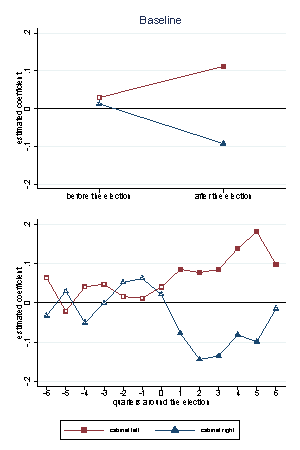
\includegraphics[width=\linewidth]{../results/applications/app_graphs_baseline.pdf}
%		{\footnotesize Note: These figures show the time evolution of refugee inflows as estimated in fixed effects regression with a set of dummies for before and after the election or a set of dummies for different quarters before and after an election in a quarter t = 0. Significant coefficients are indicated by filled plot markers.\par}
%	\end{minipage}
%\end{figure}
%
%\clearpage
%\FloatBarrier
%\begin{table}[htbp]\centering
\def\sym#1{\ifmmode^{#1}\else\(^{#1}\)\fi}
\caption{Coefficients Graph 2}
\begin{tabular}{l*{2}{c}}
\hline\hline
                    &\multicolumn{1}{c}{(1)}&\multicolumn{1}{c}{(2)}\\
                    &\multicolumn{1}{c}{left}&\multicolumn{1}{c}{right}\\
\hline
 6 quarters before the election&      0.0555\sym{*}  &     -0.0244         \\
                    &    (0.0275)         &    (0.0365)         \\
[1em]
 5 quarters before the election&     -0.0294         &      0.0385         \\
                    &    (0.0295)         &    (0.0311)         \\
[1em]
 4 quarters before the election&      0.0333         &     -0.0422         \\
                    &    (0.0366)         &    (0.0385)         \\
[1em]
 3 quarters before the election&      0.0398         &     0.00650         \\
                    &    (0.0439)         &    (0.0302)         \\
[1em]
 2 quarters before the election&     0.00828         &      0.0600         \\
                    &    (0.0358)         &    (0.0385)         \\
[1em]
 1 quarters before the election&     0.00414         &      0.0701         \\
                    &    (0.0425)         &    (0.0363)         \\
[1em]
Quarter of the election&      0.0325         &      0.0293         \\
                    &    (0.0393)         &    (0.0374)         \\
[1em]
 1 quarters after the election&      0.0775\sym{*}  &     -0.0698         \\
                    &    (0.0373)         &    (0.0364)         \\
[1em]
 2 quarters after the election&      0.0697\sym{*}  &      -0.136\sym{***}\\
                    &    (0.0346)         &    (0.0338)         \\
[1em]
 3 quarters after the election&      0.0774\sym{*}  &      -0.127\sym{**} \\
                    &    (0.0339)         &    (0.0448)         \\
[1em]
 4 quarters after the election&       0.131\sym{***}&     -0.0733         \\
                    &    (0.0315)         &    (0.0384)         \\
[1em]
 5 quarters after the election&       0.173\sym{***}&     -0.0904\sym{**} \\
                    &    (0.0288)         &    (0.0350)         \\
[1em]
 6 quarters after the election&      0.0899\sym{***}&    -0.00688         \\
                    &    (0.0264)         &    (0.0296)         \\
\hline
Observations        &       23705         &       23705         \\
\hline\hline
\multicolumn{3}{l}{\footnotesize Standard errors in parentheses}\\
\multicolumn{3}{l}{\footnotesize \sym{*} \(p<0.05\), \sym{**} \(p<0.01\), \sym{***} \(p<0.001\)}\\
\end{tabular}
\end{table}



\clearpage
\FloatBarrier
\begin{figure}[!ht]
	\caption{First-time asylum applications per capita: predicted pattern - R1 to R6}
	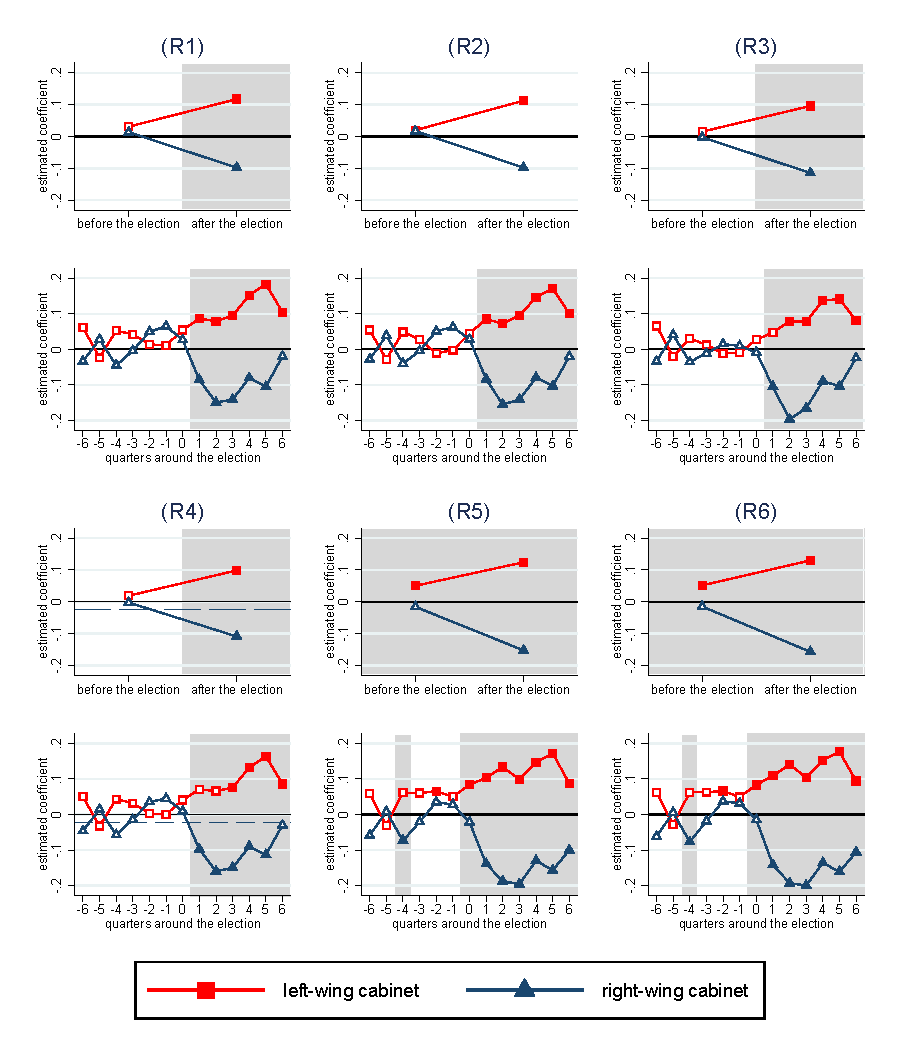
\includegraphics[width=1\textwidth]{../results/applications/app_graphs_R1-R6.pdf}
	\footnotesize{Note: These figures show the time evolution of refugee inflows as estimated in fixed effects regression
		with a set of dummies for before and after the election or a set of dummies for different quarters before and after an election in a quarter t = 0. Significant coefficients are indicated by filled plot markers. The dashed line in subfigure R4 shows the average inflow of asylum seekers under right-wing cabinets in periods outside the election period. Significance of the coefficients is reported for the distance to this average non-election period effect.}
\end{figure}

\clearpage
\FloatBarrier

\begin{table}[htbp]\centering
\def\sym#1{\ifmmode^{#1}\else\(^{#1}\)\fi}
\caption{Coefficients R1 - R3}
\begin{tabular}{l*{6}{c}}
\hline\hline
                    &\multicolumn{1}{c}{(1)}&\multicolumn{1}{c}{(2)}&\multicolumn{1}{c}{(3)}&\multicolumn{1}{c}{(4)}&\multicolumn{1}{c}{(5)}&\multicolumn{1}{c}{(6)}\\
                    &\multicolumn{1}{c}{left\_R1}&\multicolumn{1}{c}{right\_R1}&\multicolumn{1}{c}{left\_R2}&\multicolumn{1}{c}{right\_R2}&\multicolumn{1}{c}{left\_R3}&\multicolumn{1}{c}{right\_R3}\\
\hline
 6 quarters before the election&      0.0517         &     -0.0187         &      0.0495         &     -0.0184         &      0.0692\sym{*}  &     -0.0346         \\
                    &    (0.0283)         &    (0.0369)         &    (0.0280)         &    (0.0364)         &    (0.0276)         &    (0.0368)         \\
[1em]
 5 quarters before the election&     -0.0356         &      0.0450         &     -0.0345         &      0.0507         &     -0.0170         &      0.0408         \\
                    &    (0.0305)         &    (0.0313)         &    (0.0300)         &    (0.0307)         &    (0.0296)         &    (0.0310)         \\
[1em]
 4 quarters before the election&      0.0289         &     -0.0371         &      0.0304         &     -0.0371         &      0.0255         &     -0.0415         \\
                    &    (0.0377)         &    (0.0389)         &    (0.0363)         &    (0.0388)         &    (0.0362)         &    (0.0388)         \\
[1em]
 3 quarters before the election&      0.0353         &     0.00854         &      0.0255         &     0.00329         &      0.0184         &     -0.0141         \\
                    &    (0.0449)         &    (0.0312)         &    (0.0444)         &    (0.0318)         &    (0.0431)         &    (0.0302)         \\
[1em]
 2 quarters before the election&     0.00504         &      0.0661         &     -0.0148         &      0.0633         &    -0.00509         &      0.0145         \\
                    &    (0.0368)         &    (0.0394)         &    (0.0360)         &    (0.0397)         &    (0.0355)         &    (0.0375)         \\
[1em]
 1 quarters before the election&    0.000175         &      0.0817\sym{*}  &    -0.00881         &      0.0745\sym{*}  &    -0.00515         &     0.00946         \\
                    &    (0.0429)         &    (0.0378)         &    (0.0426)         &    (0.0366)         &    (0.0421)         &    (0.0367)         \\
[1em]
Quarter of the election&      0.0313         &      0.0382         &      0.0268         &      0.0356         &      0.0237         &     -0.0119         \\
                    &    (0.0388)         &    (0.0380)         &    (0.0384)         &    (0.0379)         &    (0.0384)         &    (0.0378)         \\
[1em]
 1 quarters after the election&      0.0792\sym{*}  &     -0.0659         &      0.0821\sym{*}  &     -0.0693         &      0.0551         &      -0.104\sym{**} \\
                    &    (0.0365)         &    (0.0368)         &    (0.0370)         &    (0.0356)         &    (0.0365)         &    (0.0365)         \\
[1em]
 2 quarters after the election&      0.0683\sym{*}  &      -0.133\sym{***}&      0.0663\sym{*}  &      -0.144\sym{***}&      0.0820\sym{*}  &      -0.198\sym{***}\\
                    &    (0.0341)         &    (0.0338)         &    (0.0338)         &    (0.0333)         &    (0.0332)         &    (0.0332)         \\
[1em]
 3 quarters after the election&      0.0827\sym{*}  &      -0.125\sym{**} &      0.0877\sym{**} &      -0.131\sym{**} &      0.0801\sym{*}  &      -0.168\sym{***}\\
                    &    (0.0334)         &    (0.0451)         &    (0.0332)         &    (0.0435)         &    (0.0332)         &    (0.0451)         \\
[1em]
 4 quarters after the election&       0.136\sym{***}&     -0.0710         &       0.135\sym{***}&     -0.0749         &       0.137\sym{***}&     -0.0954\sym{*}  \\
                    &    (0.0310)         &    (0.0388)         &    (0.0316)         &    (0.0383)         &    (0.0308)         &    (0.0384)         \\
[1em]
 5 quarters after the election&       0.177\sym{***}&     -0.0888\sym{*}  &       0.170\sym{***}&     -0.0925\sym{**} &       0.149\sym{***}&      -0.106\sym{**} \\
                    &    (0.0291)         &    (0.0357)         &    (0.0284)         &    (0.0346)         &    (0.0286)         &    (0.0351)         \\
[1em]
 6 quarters after the election&      0.0923\sym{***}&    -0.00404         &      0.0935\sym{**} &    -0.00948         &      0.0833\sym{**} &     -0.0251         \\
                    &    (0.0268)         &    (0.0303)         &    (0.0285)         &    (0.0301)         &    (0.0262)         &    (0.0292)         \\
\hline
Observations        &       23705         &       23705         &       23705         &       23705         &       23705         &       23705         \\
\hline\hline
\multicolumn{7}{l}{\footnotesize Standard errors in parentheses}\\
\multicolumn{7}{l}{\footnotesize \sym{*} \(p<0.05\), \sym{**} \(p<0.01\), \sym{***} \(p<0.001\)}\\
\end{tabular}
\end{table}

\begin{table}[htbp]\centering
\def\sym#1{\ifmmode^{#1}\else\(^{#1}\)\fi}
\caption{Coefficients R4 - R6}
\begin{tabular}{l*{6}{c}}
\hline\hline
                    &\multicolumn{1}{c}{(1)}&\multicolumn{1}{c}{(2)}&\multicolumn{1}{c}{(3)}&\multicolumn{1}{c}{(4)}&\multicolumn{1}{c}{(5)}&\multicolumn{1}{c}{(6)}\\
                    &\multicolumn{1}{c}{left\_R4}&\multicolumn{1}{c}{right\_R4}&\multicolumn{1}{c}{left\_R5}&\multicolumn{1}{c}{right\_R5}&\multicolumn{1}{c}{left\_R6}&\multicolumn{1}{c}{right\_R6}\\
\hline
 6 quarters before the election&      0.0638         &     -0.0326         &      0.0307         &     -0.0247         &      0.0285         &     -0.0219         \\
                    &    (0.0340)         &    (0.0415)         &    (0.0277)         &    (0.0365)         &    (0.0275)         &    (0.0368)         \\
[1em]
 5 quarters before the election&     -0.0213         &      0.0301         &     -0.0608\sym{*}  &      0.0455         &     -0.0629\sym{*}  &      0.0489         \\
                    &    (0.0313)         &    (0.0346)         &    (0.0302)         &    (0.0316)         &    (0.0303)         &    (0.0320)         \\
[1em]
 4 quarters before the election&      0.0411         &     -0.0504         &      0.0186         &     -0.0476         &      0.0131         &     -0.0459         \\
                    &    (0.0341)         &    (0.0370)         &    (0.0372)         &    (0.0385)         &    (0.0377)         &    (0.0386)         \\
[1em]
 3 quarters before the election&      0.0477         &    -0.00112         &      0.0369         &     0.00921         &      0.0341         &      0.0181         \\
                    &    (0.0414)         &    (0.0299)         &    (0.0441)         &    (0.0306)         &    (0.0439)         &    (0.0323)         \\
[1em]
 2 quarters before the election&      0.0161         &      0.0522         &      0.0403         &      0.0710         &      0.0345         &      0.0802\sym{*}  \\
                    &    (0.0336)         &    (0.0373)         &    (0.0353)         &    (0.0390)         &    (0.0355)         &    (0.0393)         \\
[1em]
 1 quarters before the election&      0.0122         &      0.0623         &      0.0212         &      0.0632         &      0.0142         &      0.0746\sym{*}  \\
                    &    (0.0363)         &    (0.0342)         &    (0.0418)         &    (0.0363)         &    (0.0415)         &    (0.0373)         \\
[1em]
Quarter of the election&      0.0406         &      0.0215         &      0.0407         &     0.00853         &      0.0336         &      0.0228         \\
                    &    (0.0362)         &    (0.0385)         &    (0.0385)         &    (0.0373)         &    (0.0384)         &    (0.0378)         \\
[1em]
 1 quarters after the election&      0.0853\sym{*}  &     -0.0777\sym{*}  &      0.0790\sym{*}  &     -0.0989\sym{**} &      0.0799\sym{*}  &     -0.0957\sym{**} \\
                    &    (0.0390)         &    (0.0324)         &    (0.0374)         &    (0.0371)         &    (0.0379)         &    (0.0368)         \\
[1em]
 2 quarters after the election&      0.0775\sym{*}  &      -0.144\sym{***}&       0.106\sym{**} &      -0.151\sym{***}&       0.106\sym{**} &      -0.149\sym{***}\\
                    &    (0.0303)         &    (0.0353)         &    (0.0355)         &    (0.0340)         &    (0.0368)         &    (0.0333)         \\
[1em]
 3 quarters after the election&      0.0852\sym{**} &      -0.136\sym{***}&      0.0692\sym{*}  &      -0.160\sym{***}&      0.0681\sym{*}  &      -0.157\sym{***}\\
                    &    (0.0324)         &    (0.0391)         &    (0.0337)         &    (0.0450)         &    (0.0340)         &    (0.0463)         \\
[1em]
 4 quarters after the election&       0.139\sym{***}&     -0.0814\sym{*}  &       0.113\sym{***}&      -0.102\sym{**} &       0.111\sym{***}&      -0.102\sym{**} \\
                    &    (0.0278)         &    (0.0345)         &    (0.0313)         &    (0.0385)         &    (0.0326)         &    (0.0385)         \\
[1em]
 5 quarters after the election&       0.181\sym{***}&     -0.0990\sym{**} &       0.148\sym{***}&      -0.120\sym{***}&       0.146\sym{***}&      -0.117\sym{***}\\
                    &    (0.0277)         &    (0.0356)         &    (0.0288)         &    (0.0357)         &    (0.0289)         &    (0.0345)         \\
[1em]
 6 quarters after the election&      0.0985\sym{**} &     -0.0149         &      0.0568\sym{*}  &     -0.0657\sym{*}  &      0.0568\sym{*}  &     -0.0646\sym{*}  \\
                    &    (0.0301)         &    (0.0302)         &    (0.0258)         &    (0.0305)         &    (0.0264)         &    (0.0302)         \\
\hline
Observations        &       23705         &       23705         &       23705         &       23705         &       23705         &       23705         \\
\hline\hline
\multicolumn{7}{l}{\footnotesize Standard errors in parentheses}\\
\multicolumn{7}{l}{\footnotesize \sym{*} \(p<0.05\), \sym{**} \(p<0.01\), \sym{***} \(p<0.001\)}\\
\end{tabular}
\end{table}



\clearpage
\FloatBarrier
\begin{table}[htbp]\centering \footnotesize
\def\sym#1{\ifmmode^{#1}\else\(^{#1}\)\fi}
\caption{Determinants of first-time asylum applications per capita - R7 - R12}
\begin{tabular}{l*{6}{c}}
\hline\hline
	&\multicolumn{1}{c}{(1)}     &\multicolumn{1}{c}{(2)}       &\multicolumn{1}{c}{(3)}       &\multicolumn{1}{c}{(4)}    	&\multicolumn{1}{c}{(5)}  	&\multicolumn{1}{c}{(6)}   \\
                    &\multicolumn{1}{c}{R7}         &\multicolumn{1}{c}{R8}         &\multicolumn{1}{c}{R9}         &\multicolumn{1}{c}{R10}         &\multicolumn{1}{c}{R11}         &\multicolumn{1}{c}{R12}         \\
\hline
Political Terror Scale	&       0.400\sym{***}& 0.337\sym{***}    &       0.409\sym{***}&       0.400\sym{***}&       0.400\sym{***}&       0.404\sym{***}\\
                    	&    (0.0696)         &     (0.0616)                  &    (0.0696)         &    (0.0697)         &    (0.0450)         &    (0.0706)         \\
[0,5em]
Civic Liberty (FHI) 	&       0.142         &        0.129              &       0.176         &       0.175         &       0.175\sym{**} &       0.170         \\
                    	&     (0.127)         &        (0.123)             &     (0.129)         &     (0.131)         &    (0.0611)         &     (0.134)         \\
[0,5em]
Political Rights (FHI)	&      0.0633         &       0.0564                &      0.0450         &      0.0487         &      0.0487         &      0.0476         \\
                    	&    (0.0712)         &          (0.0670)           &    (0.0751)         &    (0.0752)         &    (0.0479)         &    (0.0758)         \\
[0,5em]
Quarterly civil war 	&       0.192\sym{***}&     0.160\sym{***}          &    0.126\sym{***}                 &       0.188\sym{***}&       0.188\sym{***}&       0.186\sym{***}\\
battle death (000s)     &    (0.0224)         &  (0.0221)                   &     (0.0139)                 &    (0.0234)         &    (0.0265)         &    (0.0236)         \\
[0,5em]
Log origin country 		&      -0.636\sym{***}&   -0.693\sym{***}                  &      -0.654\sym{***}&      -0.661\sym{***}&      -0.661\sym{***}&      -0.651\sym{***}\\
real GDP per capita     &     (0.158)         &     (0.149)                 &     (0.167)         &     (0.163)         &     (0.105)         &     (0.163)         \\
[0,5em]
Log destination country &      -1.484\sym{**} &      -1.447\sym{**} &      -1.464\sym{**} &      -1.470\sym{**} &      -1.470\sym{*}  &      -1.483\sym{**} \\
real GDP per capita     &     (0.443)         &     (0.439)         &     (0.440)         &     (0.440)         &     (0.608)         &     (0.443)         \\
[0,5em]
Quarterly unemployment &     -0.0714\sym{***}&     -0.0740\sym{***}&     -0.0744\sym{***}&     -0.0745\sym{***}&     -0.0745\sym{***}&     -0.0714\sym{***}\\
rate at destination    &    (0.0108)         &    (0.0108)         &    (0.0108)         &    (0.0108)         &    (0.0112)         &    (0.0108)         \\
[0,5em]
Years after 2007          &                     &                     &                     &       0.190         &                     &                     \\
                    &                     &                     &                     &     (0.183)         &                     &                     \\
[0,5em]
Cabinet position left * &      0.0357         &      0.0290         &      0.0288         &      0.0291         &      0.0291         &      0.0248         \\
Before the election                    &    (0.0245)         &    (0.0245)         &    (0.0244)         &    (0.0244)         &    (0.0301)         &    (0.0240)         \\
[0,5em]
Cabinet position left * &       0.115\sym{***}&       0.112\sym{***}&       0.112\sym{***}&       0.112\sym{***}&       0.112\sym{***}&      0.0993\sym{***}\\
After the election                    &    (0.0215)         &    (0.0216)         &    (0.0215)         &    (0.0215)         &    (0.0286)         &    (0.0220)         \\
[0,5em]
Cabinet position right * &     0.00861         &      0.0120         &      0.0128         &      0.0128         &      0.0128         &      0.0135         \\
Before the election                    &    (0.0234)         &    (0.0234)         &    (0.0235)         &    (0.0234)         &    (0.0302)         &    (0.0238)         \\
[0,5em]
Cabinet position right * &     -0.0945\sym{***}&     -0.0945\sym{***}&     -0.0923\sym{***}&     -0.0929\sym{***}&     -0.0929\sym{**} &     -0.0913\sym{***}\\
After the election                    &    (0.0225)         &    (0.0223)         &    (0.0227)         &    (0.0226)         &    (0.0303)         &    (0.0261)         \\
\hline
Observations        &       23705         &       23705         &       23705         &       23705         &       23705         &       23239         \\
Adjusted \(R^{2}\)  &       0.182         &       0.168         &       0.177         &       0.176         &       0.176         &       0.175         \\
Fixed Effects       &       D x O         &       D x O         &       D x O         &       D x O         &       D x O         &       D x O         \\
Destination dummies &          No         &          No         &          No         &          No         &          No         &          No         \\
Quarter-Year dummies&         Yes         &         Yes         &         Yes         &         Yes         &         Yes         &         Yes         \\
\hline\hline
\multicolumn{7}{l}{Standard errors in parentheses \sym{*} \(p<0.05\), \sym{**} \(p<0.01\), \sym{***} \(p<0.001\)}\\
\end{tabular}
\end{table}


\clearpage
\FloatBarrier
\begin{figure}[!ht]
	\caption{First-time asylum applications per capita: predicted pattern - R7 to R12}
	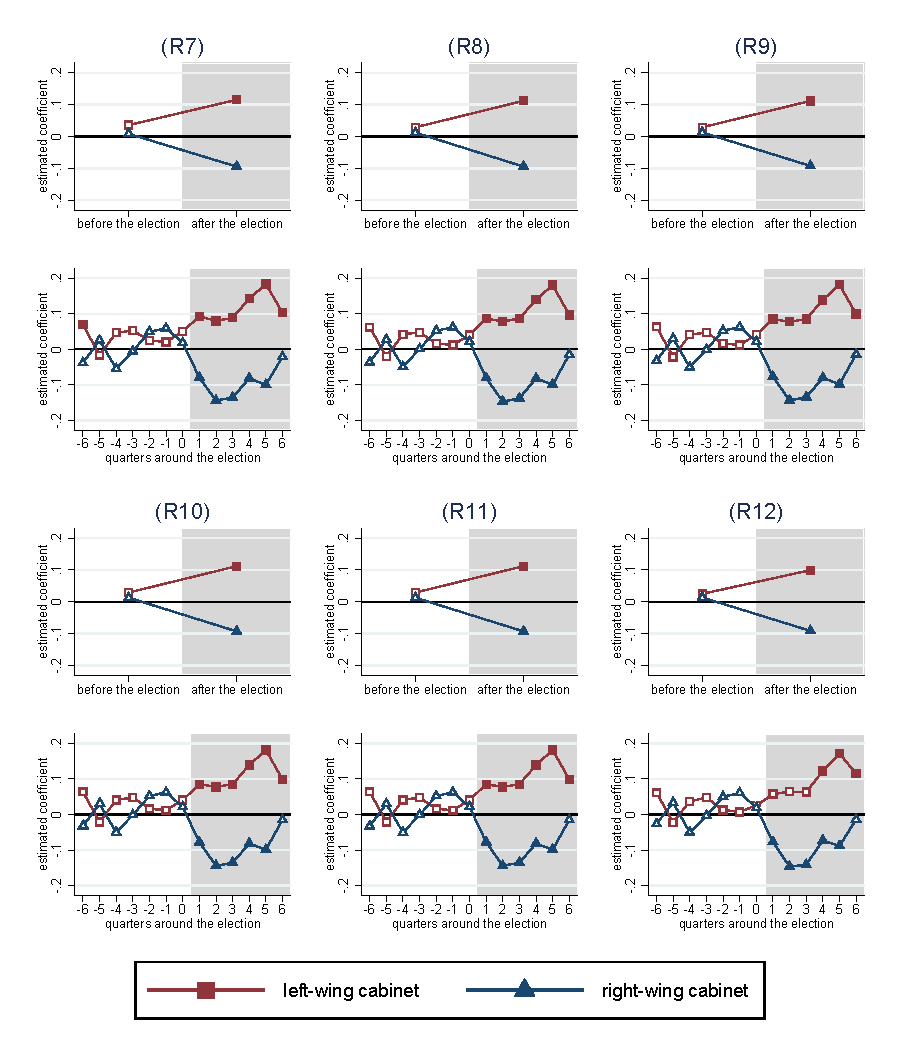
\includegraphics[width=1\textwidth]{../results/applications/app_graphs_R7-R12.pdf}
	\footnotesize{Note: These figures show the time evolution of refugee inflows as estimated in fixed effects regression
		with a set of dummies for before and after the election or a set of dummies for different quarters before and after an election in a quarter t = 0. Significant coefficients are indicated by filled plot markers.}
\end{figure}

\clearpage
\FloatBarrier

\begin{table}[!ht]\centering \scriptsize
\def\sym#1{\ifmmode^{#1}\else\(^{#1}\)\fi}
\caption{Coefficients quarterly model - R7 - R9}
\begin{tabular}{l*{6}{c}}
\hline\hline
                    &\multicolumn{2}{c}{(R7)}&\multicolumn{2}{c}{(R8)}&\multicolumn{2}{c}{(R9)}\\
                    &\multicolumn{1}{c}{left}&\multicolumn{1}{c}{right}&\multicolumn{1}{c}{left}&\multicolumn{1}{c}{right}&\multicolumn{1}{c}{left}&\multicolumn{1}{c}{right}\\
\hline
 6 quarters before the election&      0.0692\sym{*}  &     -0.0383         &      0.0620         &     -0.0366         &      0.0630         &     -0.0325         \\
                    &    (0.0340)         &    (0.0415)         &    (0.0345)         &    (0.0411)         &    (0.0342)         &    (0.0414)         \\
[0,12em]
 5 quarters before the election&     -0.0167         &      0.0254         &     -0.0207         &      0.0276         &     -0.0218         &      0.0301         \\
                    &    (0.0314)         &    (0.0345)         &    (0.0318)         &    (0.0346)         &    (0.0314)         &    (0.0346)         \\
[0,12em]
 4 quarters before the election&      0.0464         &     -0.0546         &      0.0421         &     -0.0496         &      0.0407         &     -0.0504         \\
                    &    (0.0341)         &    (0.0370)         &    (0.0339)         &    (0.0368)         &    (0.0340)         &    (0.0371)         \\
[0,12em]
 3 quarters before the election&      0.0528         &    -0.00540         &      0.0471         &     0.00100         &      0.0473         &    -0.00110         \\
                    &    (0.0414)         &    (0.0298)         &    (0.0414)         &    (0.0302)         &    (0.0414)         &    (0.0299)         \\
[0,12em]
 2 quarters before the election&      0.0244         &      0.0493         &      0.0164         &      0.0524         &      0.0160         &      0.0523         \\
                    &    (0.0336)         &    (0.0373)         &    (0.0336)         &    (0.0369)         &    (0.0336)         &    (0.0373)         \\
[0,12em]
 1 quarters before the election&      0.0206         &      0.0588         &      0.0118         &      0.0616         &      0.0123         &      0.0624         \\
                    &    (0.0364)         &    (0.0339)         &    (0.0364)         &    (0.0341)         &    (0.0363)         &    (0.0342)         \\
[0,12em]
Quarter of the election&      0.0498         &      0.0182         &      0.0406         &      0.0212         &      0.0408         &      0.0215         \\
                    &    (0.0363)         &    (0.0384)         &    (0.0365)         &    (0.0386)         &    (0.0361)         &    (0.0385)         \\
[0,12em]
 1 quarters after the election&      0.0926\sym{*}  &     -0.0796\sym{*}  &      0.0866\sym{*}  &     -0.0808\sym{*}  &      0.0852\sym{*}  &     -0.0775\sym{*}  \\
                    &    (0.0388)         &    (0.0322)         &    (0.0389)         &    (0.0322)         &    (0.0390)         &    (0.0324)         \\
[0,12em]
 2 quarters after the election&      0.0796\sym{**} &      -0.144\sym{***}&      0.0778\sym{*}  &      -0.147\sym{***}&      0.0771\sym{*}  &      -0.144\sym{***}\\
                    &    (0.0302)         &    (0.0352)         &    (0.0308)         &    (0.0349)         &    (0.0304)         &    (0.0354)         \\
[0,12em]
 3 quarters after the election&      0.0883\sym{**} &      -0.136\sym{***}&      0.0865\sym{**} &      -0.138\sym{***}&      0.0849\sym{**} &      -0.135\sym{***}\\
                    &    (0.0325)         &    (0.0391)         &    (0.0322)         &    (0.0394)         &    (0.0324)         &    (0.0390)         \\
[0,12em]
 4 quarters after the election&       0.142\sym{***}&     -0.0815\sym{*}  &       0.139\sym{***}&     -0.0820\sym{*}  &       0.139\sym{***}&     -0.0805\sym{*}  \\
                    &    (0.0278)         &    (0.0346)         &    (0.0282)         &    (0.0342)         &    (0.0278)         &    (0.0347)         \\
[0,12em]
 5 quarters after the election&       0.183\sym{***}&      -0.100\sym{**} &       0.181\sym{***}&     -0.0996\sym{**} &       0.182\sym{***}&     -0.0982\sym{**} \\
                    &    (0.0277)         &    (0.0356)         &    (0.0282)         &    (0.0351)         &    (0.0276)         &    (0.0358)         \\
[0,12em]
 6 quarters after the election&       0.103\sym{***}&     -0.0209         &      0.0963\sym{**} &     -0.0146         &      0.0989\sym{***}&     -0.0143         \\
                    &    (0.0301)         &    (0.0303)         &    (0.0306)         &    (0.0301)         &    (0.0300)         &    (0.0303)         \\
\hline
Observations        &       23705         &       23705         &       23705         &       23705         &       23705         &       23705         \\
\hline\hline
\multicolumn{7}{l}{ Standard errors in parentheses \sym{*} \(p<0.05\), \sym{**} \(p<0.01\), \sym{***} \(p<0.001\)}\\
\end{tabular}
\end{table}

\begin{table}[htbp]\centering
\def\sym#1{\ifmmode^{#1}\else\(^{#1}\)\fi}
\caption{Coefficients R10 - R12}
\begin{tabular}{l*{6}{c}}
\hline\hline
                    &\multicolumn{1}{c}{(1)}&\multicolumn{1}{c}{(2)}&\multicolumn{1}{c}{(3)}&\multicolumn{1}{c}{(4)}&\multicolumn{1}{c}{(5)}&\multicolumn{1}{c}{(6)}\\
                    &\multicolumn{1}{c}{left\_R10}&\multicolumn{1}{c}{right\_R10}&\multicolumn{1}{c}{left\_R11}&\multicolumn{1}{c}{right\_R11}&\multicolumn{1}{c}{left\_R12}&\multicolumn{1}{c}{right\_R12}\\
\hline
 6 quarters before the election&      0.0555\sym{*}  &     -0.0244         &      0.0229         &     0.00948         &      0.0553\sym{*}  &     -0.0210         \\
                    &    (0.0275)         &    (0.0365)         &    (0.0295)         &    (0.0332)         &    (0.0260)         &    (0.0365)         \\
[1em]
 5 quarters before the election&     -0.0294         &      0.0385         &     -0.0444         &      0.0515         &     -0.0273         &      0.0392         \\
                    &    (0.0295)         &    (0.0311)         &    (0.0325)         &    (0.0294)         &    (0.0296)         &    (0.0311)         \\
[1em]
 4 quarters before the election&      0.0333         &     -0.0422         &      0.0277         &     -0.0390         &      0.0317         &     -0.0445         \\
                    &    (0.0366)         &    (0.0385)         &    (0.0375)         &    (0.0375)         &    (0.0367)         &    (0.0383)         \\
[1em]
 3 quarters before the election&      0.0398         &     0.00650         &      0.0286         &      0.0146         &      0.0420         &     0.00156         \\
                    &    (0.0439)         &    (0.0302)         &    (0.0433)         &    (0.0318)         &    (0.0441)         &    (0.0303)         \\
[1em]
 2 quarters before the election&     0.00828         &      0.0600         &      0.0129         &      0.0620         &     0.00741         &      0.0550         \\
                    &    (0.0358)         &    (0.0385)         &    (0.0352)         &    (0.0395)         &    (0.0361)         &    (0.0388)         \\
[1em]
 1 quarters before the election&     0.00414         &      0.0701         &      0.0136         &      0.0657         &     0.00189         &      0.0660         \\
                    &    (0.0425)         &    (0.0363)         &    (0.0415)         &    (0.0373)         &    (0.0436)         &    (0.0360)         \\
[1em]
Quarter of the election&      0.0325         &      0.0293         &      0.0249         &      0.0394         &      0.0198         &      0.0254         \\
                    &    (0.0393)         &    (0.0374)         &    (0.0400)         &    (0.0374)         &    (0.0407)         &    (0.0373)         \\
[1em]
 1 quarters after the election&      0.0775\sym{*}  &     -0.0698         &      0.0678         &     -0.0709\sym{*}  &      0.0520         &     -0.0719         \\
                    &    (0.0373)         &    (0.0364)         &    (0.0366)         &    (0.0347)         &    (0.0387)         &    (0.0373)         \\
[1em]
 2 quarters after the election&      0.0697\sym{*}  &      -0.136\sym{***}&      0.0728\sym{*}  &      -0.139\sym{***}&      0.0591         &      -0.141\sym{***}\\
                    &    (0.0346)         &    (0.0338)         &    (0.0358)         &    (0.0346)         &    (0.0378)         &    (0.0339)         \\
[1em]
 3 quarters after the election&      0.0774\sym{*}  &      -0.127\sym{**} &      0.0860\sym{*}  &      -0.126\sym{**} &      0.0578         &      -0.135\sym{**} \\
                    &    (0.0339)         &    (0.0448)         &    (0.0358)         &    (0.0418)         &    (0.0348)         &    (0.0493)         \\
[1em]
 4 quarters after the election&       0.131\sym{***}&     -0.0733         &       0.142\sym{***}&     -0.0720         &       0.117\sym{***}&     -0.0672         \\
                    &    (0.0315)         &    (0.0384)         &    (0.0345)         &    (0.0385)         &    (0.0322)         &    (0.0424)         \\
[1em]
 5 quarters after the election&       0.173\sym{***}&     -0.0904\sym{**} &       0.163\sym{***}&     -0.0641         &       0.166\sym{***}&     -0.0826\sym{*}  \\
                    &    (0.0288)         &    (0.0350)         &    (0.0314)         &    (0.0332)         &    (0.0291)         &    (0.0360)         \\
[1em]
 6 quarters after the election&      0.0899\sym{***}&    -0.00688         &       0.103\sym{***}&     -0.0160         &       0.109\sym{***}&    -0.00823         \\
                    &    (0.0264)         &    (0.0296)         &    (0.0279)         &    (0.0310)         &    (0.0293)         &    (0.0309)         \\
\hline
Observations        &       23705         &       23705         &       23705         &       23705         &       23239         &       23239         \\
\hline\hline
\multicolumn{7}{l}{\footnotesize Standard errors in parentheses}\\
\multicolumn{7}{l}{\footnotesize \sym{*} \(p<0.05\), \sym{**} \(p<0.01\), \sym{***} \(p<0.001\)}\\
\end{tabular}
\end{table}


\clearpage
\FloatBarrier
\begin{table}[htbp]\centering \scriptsize
\def\sym#1{\ifmmode^{#1}\else\(^{#1}\)\fi}
\caption{Determinants of first-time asylum applications per capita - R13 - R18}
\begin{tabular}{l*{6}{c}}
\hline\hline
	&\multicolumn{1}{c}{(1)}     &\multicolumn{1}{c}{(2)}       &\multicolumn{1}{c}{(3)}       &\multicolumn{1}{c}{(4)}    	&\multicolumn{1}{c}{(5)}  	&\multicolumn{1}{c}{(6)}   \\
                    &\multicolumn{1}{c}{R13}         &\multicolumn{1}{c}{R14}         &\multicolumn{1}{c}{R15}         &\multicolumn{1}{c}{R16}         &\multicolumn{1}{c}{R17}         &\multicolumn{1}{c}{R18}         \\
\hline
Political Terror Scale&       0.400\sym{***}&       0.400\sym{***}&       0.374\sym{***}&       0.414\sym{***}&       0.404\sym{***}&       0.410\sym{***}\\
                    &    (0.0450)         &    (0.0450)         &    (0.0657)         &    (0.0750)         &    (0.0785)         &    (0.0849)         \\
[0.5em]
Civic Liberty (FHI) &       0.175\sym{**} &       0.176\sym{**} &       0.166         &       0.195         &       0.163         &       0.172         \\
                    &    (0.0611)         &    (0.0612)         &     (0.124)         &     (0.133)         &     (0.132)         &     (0.143)         \\
[0.5em]
Political Rights (FHI)&      0.0483         &      0.0478         &      0.0396         &      0.0420         &      0.0450         &      0.0513         \\
                    &    (0.0478)         &    (0.0478)         &    (0.0689)         &    (0.0797)         &    (0.0759)         &    (0.0785)         \\
[0.5em]
Quarterly civil war&       0.188\sym{***}&       0.187\sym{***}&       0.191\sym{***}&       0.201\sym{***}&       0.207\sym{***}&       0.186\sym{***}\\
 battle death (000s)                    &    (0.0265)         &    (0.0265)         &    (0.0226)         &    (0.0249)         &    (0.0263)         &    (0.0232)         \\
[0.5em]
Log origin country &      -0.662\sym{***}&      -0.663\sym{***}&      -0.633\sym{***}&      -0.641\sym{***}&      -0.571\sym{**} &      -0.766\sym{***}\\
real GDP per capita                   &     (0.105)         &     (0.105)         &     (0.150)         &     (0.160)         &     (0.163)         &     (0.170)         \\
[0.5em]
Log destination country &      -1.466\sym{*}  &      -1.513\sym{*}  &      -1.246\sym{**} &      -1.353\sym{*}  &      -0.102         &      -1.771\sym{***}\\
quarterly real GDP per capita                    &     (0.613)         &     (0.608)         &     (0.411)         &     (0.524)         &     (0.530)         &     (0.471)         \\
[0.5em]
Quarterly unemployment &     -0.0728\sym{***}&     -0.0736\sym{***}&     -0.0631\sym{***}&     -0.0739\sym{***}&    -0.00992         &     -0.0737\sym{***}\\
rate at destination                    &    (0.0111)         &    (0.0111)         &   (0.00955)         &    (0.0115)         &    (0.0104)         &    (0.0112)         \\
[0.5em]
Log average total first-time &                     &                     &                     &                     &       0.728\sym{***}&                     \\
applications in the previous 6 quarters                    &                     &                     &                     &                     &    (0.0524)         &                     \\
[0.5em]
Cabinet position left * &      0.0115         &      0.0143         &      0.0305         &      0.0128         &    -0.00704         &      0.0364         \\
Before the election                    &    (0.0297)         &    (0.0321)         &    (0.0229)         &    (0.0250)         &    (0.0237)         &    (0.0324)         \\
[0.5em]
Cabinet position left * &       0.104\sym{***}&       0.112\sym{***}&       0.108\sym{***}&       0.105\sym{***}&      0.0487\sym{*}  &       0.195\sym{***}\\
After the election                    &    (0.0280)         &    (0.0337)         &    (0.0203)         &    (0.0206)         &    (0.0185)         &    (0.0316)         \\
[0.5em]
Cabinet position right * &      0.0318         &      0.0322         &     0.00798         &      0.0209         &     -0.0141         &      0.0306         \\
Before the election                   &    (0.0303)         &    (0.0280)         &    (0.0213)         &    (0.0257)         &    (0.0251)         &    (0.0305)         \\
[0.5em]
Cabinet position right * &     -0.0806\sym{**} &     -0.0424         &     -0.0763\sym{**} &     -0.0992\sym{***}&     -0.0566\sym{*}  &     -0.0419         \\
After the election                    &    (0.0287)         &    (0.0276)         &    (0.0226)         &    (0.0238)         &    (0.0241)         &    (0.0319)         \\
\hline
Observations        &       23705         &       23705         &       25466         &       22446         &       22391         &       16488         \\
Adjusted \(R^{2}\)  &       0.176         &       0.175         &       0.162         &       0.185         &       0.250         &       0.183         \\
Fixed Effects       &       D x O         &       D x O         &       D x O         &       D x O         &       D x O         &       D x O         \\
Destination dummies &          No         &          No         &          No         &          No         &          No         &          No         \\
Quarter-Year dummies&         Yes         &         Yes         &         Yes         &         Yes         &         Yes         &         Yes         \\
\hline\hline
\multicolumn{7}{l}{ Standard errors in parentheses \sym{*} \(p<0.05\), \sym{**} \(p<0.01\), \sym{***} \(p<0.001\)}\\
\end{tabular}
\end{table}


\clearpage
\FloatBarrier
\begin{figure}[!ht]
	\caption{First-time asylum applications per capita: predicted pattern - R13 to R18}
	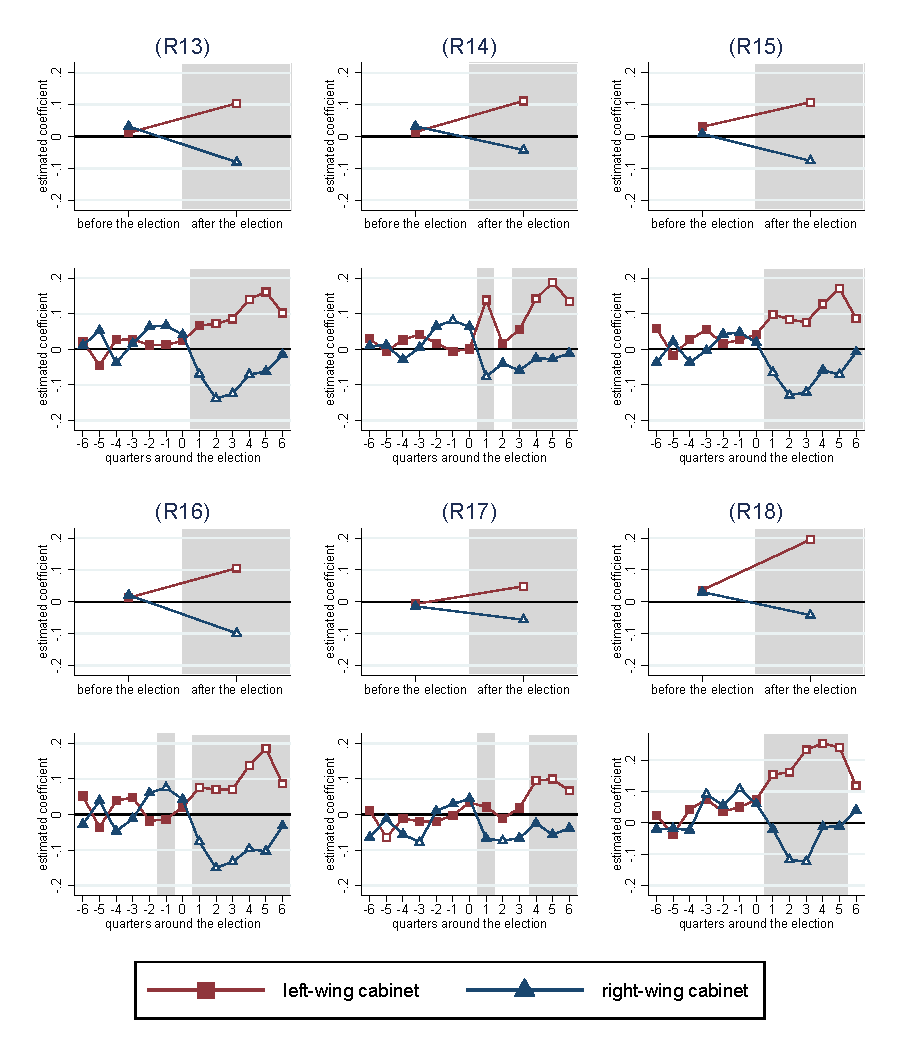
\includegraphics[width=1\textwidth]{../results/applications/app_graphs_R13-R18.pdf}
	\footnotesize{Note: These figures show the time evolution of refugee inflows as estimated in fixed effects regression
		with a set of dummies for before and after the election or a set of dummies for different quarters before and after an election in a quarter t = 0. Significant coefficients are indicated by filled plot markers.}
\end{figure}

\clearpage
\FloatBarrier

\begin{table}[!ht]\centering \scriptsize
\def\sym#1{\ifmmode^{#1}\else\(^{#1}\)\fi}
\caption{Coefficients quarterly model - R13 - R15}
\begin{tabular}{l*{6}{c}}
\hline\hline
                    &\multicolumn{2}{c}{(R13)}&\multicolumn{2}{c}{(R14)}&\multicolumn{2}{c}{(R15)}\\
&\multicolumn{1}{c}{left}&\multicolumn{1}{c}{right}&\multicolumn{1}{c}{left}&\multicolumn{1}{c}{right}&\multicolumn{1}{c}{left}&\multicolumn{1}{c}{right}\\
\hline
 6 quarters before the election&      0.0217         &      0.0106         &      0.0293         &     0.00913         &      0.0587         &     -0.0376         \\
                    &    (0.0353)         &    (0.0388)         &    (0.0375)         &    (0.0303)         &    (0.0310)         &    (0.0380)         \\
[0,12em]
 5 quarters before the election&     -0.0456         &      0.0526         &    -0.00617         &      0.0112         &     -0.0175         &      0.0212         \\
                    &    (0.0340)         &    (0.0325)         &    (0.0362)         &    (0.0286)         &    (0.0297)         &    (0.0315)         \\
[0,12em]
 4 quarters before the election&      0.0266         &     -0.0379         &      0.0262         &     -0.0299         &      0.0274         &     -0.0364         \\
                    &    (0.0336)         &    (0.0364)         &    (0.0348)         &    (0.0345)         &    (0.0311)         &    (0.0340)         \\
[0,12em]
 3 quarters before the election&      0.0275         &      0.0156         &      0.0418         &     0.00490         &      0.0548         &    -0.00400         \\
                    &    (0.0395)         &    (0.0313)         &    (0.0448)         &    (0.0283)         &    (0.0396)         &    (0.0294)         \\
[0,12em]
 2 quarters before the election&      0.0117         &      0.0631         &      0.0165         &      0.0645         &      0.0157         &      0.0424         \\
                    &    (0.0331)         &    (0.0376)         &    (0.0350)         &    (0.0368)         &    (0.0316)         &    (0.0382)         \\
[0,12em]
 1 quarters before the election&      0.0124         &      0.0668         &    -0.00546         &      0.0807\sym{*}  &      0.0267         &      0.0473         \\
                    &    (0.0361)         &    (0.0349)         &    (0.0378)         &    (0.0352)         &    (0.0351)         &    (0.0311)         \\
[0,12em]
Quarter of the election&      0.0237         &      0.0405         &    0.000592         &      0.0630         &      0.0418         &      0.0187         \\
                    &    (0.0358)         &    (0.0385)         &    (0.0415)         &    (0.0365)         &    (0.0331)         &    (0.0360)         \\
[0,12em]
 1 quarters after the election&      0.0667         &     -0.0698\sym{*}  &       0.139\sym{***}&     -0.0769\sym{*}  &      0.0980\sym{**} &     -0.0655\sym{*}  \\
                    &    (0.0371)         &    (0.0299)         &    (0.0394)         &    (0.0319)         &    (0.0357)         &    (0.0331)         \\
[0,12em]
 2 quarters after the election&      0.0717\sym{*}  &      -0.138\sym{***}&      0.0159         &     -0.0400         &      0.0841\sym{**} &      -0.129\sym{***}\\
                    &    (0.0308)         &    (0.0351)         &    (0.0330)         &    (0.0303)         &    (0.0297)         &    (0.0325)         \\
[0,12em]
 3 quarters after the election&      0.0849\sym{*}  &      -0.125\sym{***}&      0.0553         &     -0.0596         &      0.0754\sym{*}  &      -0.121\sym{**} \\
                    &    (0.0334)         &    (0.0354)         &    (0.0370)         &    (0.0342)         &    (0.0301)         &    (0.0370)         \\
[0,12em]
 4 quarters after the election&       0.141\sym{***}&     -0.0709\sym{*}  &       0.142\sym{***}&     -0.0252         &       0.127\sym{***}&     -0.0587         \\
                    &    (0.0293)         &    (0.0328)         &    (0.0365)         &    (0.0314)         &    (0.0283)         &    (0.0353)         \\
[0,12em]
 5 quarters after the election&       0.161\sym{***}&     -0.0629         &       0.188\sym{***}&     -0.0274         &       0.170\sym{***}&     -0.0711\sym{*}  \\
                    &    (0.0271)         &    (0.0321)         &    (0.0332)         &    (0.0312)         &    (0.0283)         &    (0.0332)         \\
[0,12em]
 6 quarters after the election&       0.102\sym{***}&     -0.0149         &       0.135\sym{***}&     -0.0114         &      0.0867\sym{**} &    -0.00777         \\
                    &    (0.0310)         &    (0.0309)         &    (0.0306)         &    (0.0291)         &    (0.0284)         &    (0.0332)         \\
\hline
Observations        &       23705         &       23705         &       23705         &       23705         &       25466         &       25466         \\
\hline\hline
\multicolumn{7}{l}{ Standard errors in parentheses \sym{*} \(p<0.05\), \sym{**} \(p<0.01\), \sym{***} \(p<0.001\)}\\\end{tabular}
\end{table}

\begin{table}[!ht]\centering \scriptsize
\def\sym#1{\ifmmode^{#1}\else\(^{#1}\)\fi}
\caption{Coefficients quarterly model - R16 - R18}
\begin{tabular}{l*{6}{c}}
\hline\hline
                    &\multicolumn{2}{c}{(R16)}&\multicolumn{2}{c}{(R17)}&\multicolumn{2}{c}{(R18)}\\
&\multicolumn{1}{c}{left}&\multicolumn{1}{c}{right}&\multicolumn{1}{c}{left}&\multicolumn{1}{c}{right}&\multicolumn{1}{c}{left}&\multicolumn{1}{c}{right}\\
\hline
 6 quarters before the election&      0.0517         &     -0.0270         &                     &                     &                     &                     \\
                    &    (0.0359)         &    (0.0427)         &                     &                     &                     &                     \\
[0,12em]
 5 quarters before the election&     -0.0360         &      0.0387         &     -0.0365         &      0.0223         &                     &                     \\
                    &    (0.0322)         &    (0.0335)         &    (0.0301)         &    (0.0338)         &                     &                     \\
[0,12em]
 4 quarters before the election&      0.0385         &     -0.0468         &      0.0296         &     -0.0569         &      0.0233         &     -0.0597         \\
                    &    (0.0345)         &    (0.0393)         &    (0.0339)         &    (0.0363)         &    (0.0333)         &    (0.0349)         \\
[0,12em]
 3 quarters before the election&      0.0483         &     -0.0119         &      0.0338         &     -0.0107         &      0.0236         &     -0.0183         \\
                    &    (0.0446)         &    (0.0306)         &    (0.0414)         &    (0.0300)         &    (0.0409)         &    (0.0291)         \\
[0,12em]
 2 quarters before the election&     -0.0181         &      0.0605         &     0.00348         &      0.0415         &   -0.000450         &      0.0399         \\
                    &    (0.0329)         &    (0.0387)         &    (0.0331)         &    (0.0377)         &    (0.0316)         &    (0.0371)         \\
[0,12em]
 1 quarters before the election&     -0.0131         &      0.0755\sym{*}  &   -0.000214         &      0.0537         &    -0.00479         &      0.0460         \\
                    &    (0.0356)         &    (0.0370)         &    (0.0363)         &    (0.0340)         &    (0.0355)         &    (0.0324)         \\
[0,12em]
Quarter of the election&      0.0210         &      0.0424         &      0.0283         &      0.0125         &      0.0182         &     0.00841         \\
                    &    (0.0357)         &    (0.0461)         &    (0.0357)         &    (0.0386)         &    (0.0353)         &    (0.0364)         \\
[0,12em]
 1 quarters after the election&      0.0758\sym{*}  &     -0.0767\sym{*}  &      0.0732         &     -0.0879\sym{**} &      0.0694         &     -0.0994\sym{**} \\
                    &    (0.0382)         &    (0.0350)         &    (0.0376)         &    (0.0325)         &    (0.0371)         &    (0.0313)         \\
[0,12em]
 2 quarters after the election&      0.0708\sym{*}  &      -0.150\sym{***}&      0.0673\sym{*}  &      -0.156\sym{***}&      0.0626\sym{*}  &      -0.159\sym{***}\\
                    &    (0.0305)         &    (0.0345)         &    (0.0302)         &    (0.0346)         &    (0.0287)         &    (0.0333)         \\
[0,12em]
 3 quarters after the election&      0.0708\sym{*}  &      -0.133\sym{**} &      0.0739\sym{*}  &      -0.145\sym{***}&      0.0698\sym{*}  &      -0.151\sym{***}\\
                    &    (0.0315)         &    (0.0426)         &    (0.0320)         &    (0.0380)         &    (0.0323)         &    (0.0378)         \\
[0,12em]
 4 quarters after the election&       0.138\sym{***}&     -0.0970\sym{**} &       0.128\sym{***}&     -0.0919\sym{**} &       0.123\sym{***}&     -0.0940\sym{**} \\
                    &    (0.0278)         &    (0.0337)         &    (0.0271)         &    (0.0340)         &    (0.0268)         &    (0.0328)         \\
[0,12em]
 5 quarters after the election&       0.186\sym{***}&      -0.103\sym{**} &       0.168\sym{***}&      -0.105\sym{**} &                     &                     \\
                    &    (0.0269)         &    (0.0375)         &    (0.0264)         &    (0.0353)         &                     &                     \\
[0,12em]
 6 quarters after the election&      0.0862\sym{**} &     -0.0322         &                     &                     &                     &                     \\
                    &    (0.0293)         &    (0.0322)         &                     &                     &                     &                     \\
\hline
Observations        &       22446         &       22446         &       23705         &       23705         &       23705         &       23705         \\
\hline\hline
\multicolumn{7}{l}{ Standard errors in parentheses \sym{*} \(p<0.05\), \sym{**} \(p<0.01\), \sym{***} \(p<0.001\)}\\\end{tabular}
\end{table}


\clearpage
\FloatBarrier
\begin{table}[htbp]\centering  \footnotesize
\def\sym#1{\ifmmode^{#1}\else\(^{#1}\)\fi}
\caption{Determinants of first-time asylum applications per capita - R19 - R22}
\begin{tabular}{l*{4}{c}}
\hline\hline
                    &\multicolumn{1}{c}{(R19)}         &\multicolumn{1}{c}{(R20)}         &\multicolumn{1}{c}{(R21)}         &\multicolumn{1}{c}{(R22)}         \\
\hline
Political Terror Scale&       0.399\sym{***}&       0.399\sym{***}&       0.399\sym{***}&       0.410\sym{***}\\
                    &    (0.0696)         &    (0.0696)         &    (0.0743)         &    (0.0849)         \\
[0,5em]
Civic Liberty (FHI) &       0.175         &       0.175         &       0.155         &       0.172         \\
                    &     (0.131)         &     (0.131)         &     (0.129)         &     (0.143)         \\
[0,5em]
Political Rights (FHI)&      0.0482         &      0.0484         &      0.0453         &      0.0513         \\
                    &    (0.0749)         &    (0.0751)         &    (0.0745)         &    (0.0785)         \\
[0,5em]
Quarterly civil war&       0.188\sym{***}&       0.188\sym{***}&       0.198\sym{***}&       0.186\sym{***}\\
 battle death (000s)                    &    (0.0234)         &    (0.0234)         &    (0.0241)         &    (0.0232)         \\
[0,5em]
Log origin country &      -0.660\sym{***}&      -0.662\sym{***}&      -0.595\sym{***}&      -0.766\sym{***}\\
real GDP per capita                    &     (0.163)         &     (0.163)         &     (0.159)         &     (0.170)         \\
[0,5em]
Log destination country&      -1.494\sym{**} &      -1.472\sym{**} &      -0.264         &      -1.771\sym{***}\\
 real GDP per capita                    &     (0.439)         &     (0.439)         &     (0.439)         &     (0.471)         \\
[0,5em]
Quarterly unemployment&     -0.0750\sym{***}&     -0.0742\sym{***}&     -0.0112         &     -0.0737\sym{***}\\
 rate at destination                    &    (0.0108)         &    (0.0108)         &   (0.00953)         &    (0.0112)         \\
[0,5em]
Log average total first-time applications &                     &                     &   0.703\sym{***}                   &                     \\
 in the previous 6 quarters                    &                     &                     &     (0.0501)                 &                     \\
[0,5em]
Nationalist party in parliament&       0.246\sym{***}&                     &                     &                     \\
                    &    (0.0623)         &                     &                     &                     \\
[0,5em]
Share of nationalist parties &                     &       1.715\sym{**} &                     &                     \\
in parliament                    &                     &     (0.626)         &                     &                     \\
[0,5em]
Cabinet position left *&      0.0369         &      0.0263         &     0.00208         &      0.0364         \\
 Before the election                    &    (0.0242)         &    (0.0243)         &    (0.0233)         &    (0.0324)         \\
[0,5em]
Cabinet position left * &       0.113\sym{***}&       0.116\sym{***}&      0.0576\sym{**} &       0.195\sym{***}\\
After the election                    &    (0.0213)         &    (0.0213)         &    (0.0196)         &    (0.0316)         \\
[0,5em]
Cabinet position right * &     0.00935         &      0.0141         &     -0.0204         &      0.0306         \\
Before the election                    &    (0.0235)         &    (0.0235)         &    (0.0236)         &    (0.0305)         \\
[0,5em]
Cabinet position right *&     -0.0985\sym{***}&     -0.0877\sym{***}&     -0.0572\sym{*}  &     -0.0419         \\
 After the election                    &    (0.0228)         &    (0.0226)         &    (0.0228)         &    (0.0319)         \\
\hline
Observations        &       23705         &       23705         &       23642         &       16488         \\
Adjusted \(R^{2}\)  &       0.179         &       0.177         &       0.239         &       0.183         \\
Fixed Effects       &       D x O         &       D x O         &       D x O         &       D x O         \\
Destination dummies &          No         &          No         &          No         &          No         \\
Quarter-Year dummies&         Yes         &         Yes         &         Yes         &         Yes         \\
\hline\hline
\multicolumn{5}{l}{Standard errors in parentheses \sym{*} \(p<0.05\), \sym{**} \(p<0.01\), \sym{***} \(p<0.001\)}\\
\end{tabular}
\end{table}


\clearpage
\FloatBarrier
\begin{figure}[!ht]
	\caption{First-time asylum applications per capita: predicted pattern - R19 to R22}
	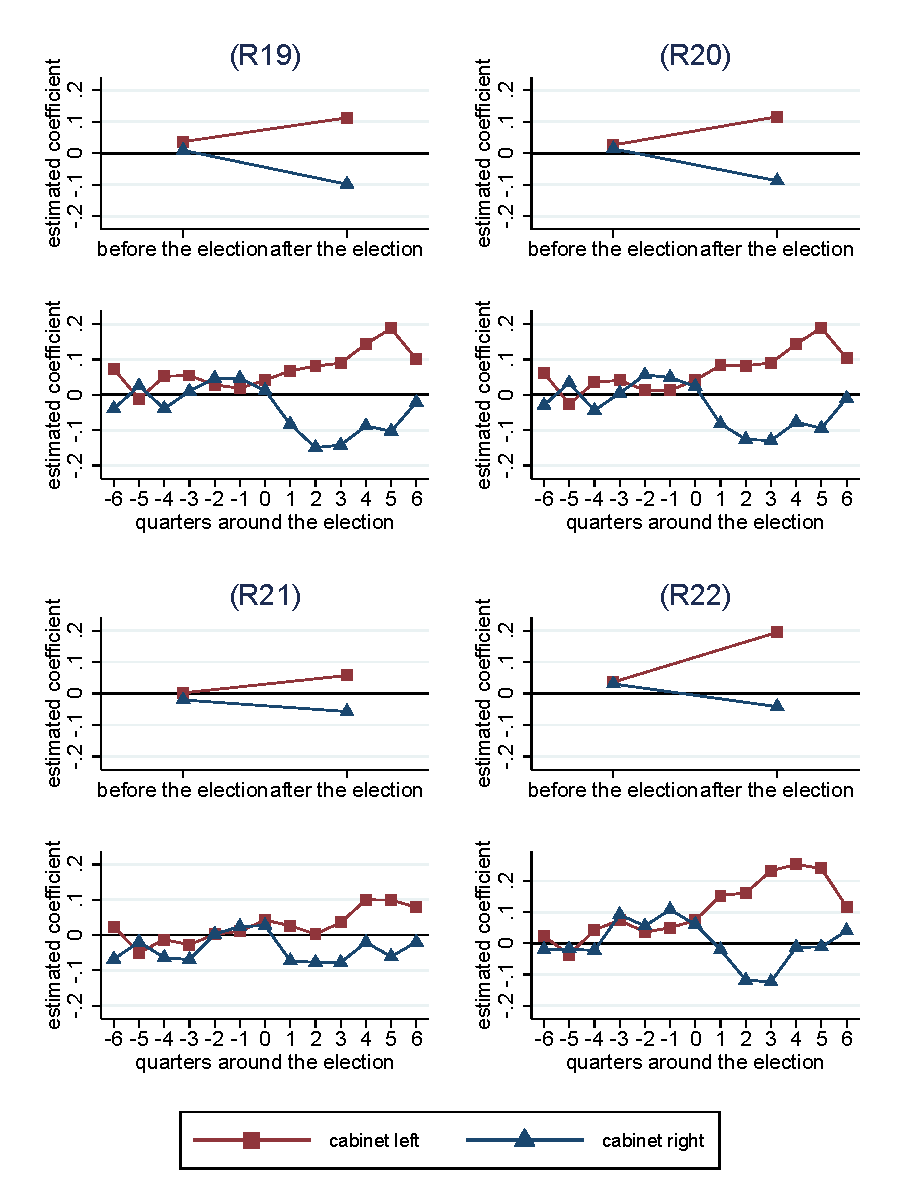
\includegraphics[width=1\textwidth]{../results/applications/app_graphs_R19-R22.pdf}
	\footnotesize{Note: These figures show the time evolution of refugee inflows as estimated in fixed effects regression
		with a set of dummies for before and after the election or a set of dummies for different quarters before and after an election in a quarter t = 0. Significant coefficients are indicated by filled plot markers.}
\end{figure}

\clearpage
\FloatBarrier

\begin{table}[!ht]\centering \scriptsize
\def\sym#1{\ifmmode^{#1}\else\(^{#1}\)\fi}
\caption{Coefficients quarterly model - R19 - R22}
\begin{tabular}{l*{8}{c}}
\hline\hline
                    &\multicolumn{2}{c}{(R19)}&\multicolumn{2}{c}{(R20)}&\multicolumn{2}{c}{(R21)}&\multicolumn{2}{c}{(R22)}\\
&\multicolumn{1}{c}{left}&\multicolumn{1}{c}{right}&\multicolumn{1}{c}{left}&\multicolumn{1}{c}{right}&\multicolumn{1}{c}{left}&\multicolumn{1}{c}{right} &\multicolumn{1}{c}{left}&\multicolumn{1}{c}{right}\\
\hline
 6 quarters before the election&      0.0735\sym{*}  &     -0.0393         &      0.0626         &     -0.0295         &      0.0135         &     -0.0263         &      0.0231         &     -0.0198         \\
                    &    (0.0336)         &    (0.0414)         &    (0.0342)         &    (0.0414)         &    (0.0303)         &    (0.0396)         &    (0.0475)         &    (0.0480)         \\
[0,12em]
 5 quarters before the election&     -0.0119         &      0.0249         &     -0.0268         &      0.0336         &     -0.0293         &      0.0350         &     -0.0368         &     -0.0180         \\
                    &    (0.0314)         &    (0.0345)         &    (0.0313)         &    (0.0347)         &    (0.0287)         &    (0.0288)         &    (0.0480)         &    (0.0362)         \\
[0,12em]
 4 quarters before the election&      0.0524         &     -0.0393         &      0.0355         &     -0.0444         &      0.0592         &     -0.0155         &      0.0429         &     -0.0230         \\
                    &    (0.0343)         &    (0.0365)         &    (0.0336)         &    (0.0367)         &    (0.0316)         &    (0.0312)         &    (0.0499)         &    (0.0402)         \\
[0,12em]
 3 quarters before the election&      0.0546         &      0.0101         &      0.0409         &     0.00487         &      0.0120         &     -0.0123         &      0.0747         &      0.0917\sym{*}  \\
                    &    (0.0413)         &    (0.0293)         &    (0.0410)         &    (0.0296)         &    (0.0297)         &    (0.0272)         &    (0.0480)         &    (0.0360)         \\
[0,12em]
 2 quarters before the election&      0.0280         &      0.0473         &      0.0134         &      0.0561         &      0.0380         &     0.00332         &      0.0358         &      0.0557         \\
                    &    (0.0336)         &    (0.0369)         &    (0.0334)         &    (0.0378)         &    (0.0287)         &    (0.0338)         &    (0.0410)         &    (0.0458)         \\
[0,12em]
 1 quarters before the election&      0.0187         &      0.0469         &      0.0128         &      0.0490         &    -0.00192         &     0.00728         &      0.0502         &       0.108\sym{*}  \\
                    &    (0.0361)         &    (0.0347)         &    (0.0364)         &    (0.0346)         &    (0.0335)         &    (0.0327)         &    (0.0467)         &    (0.0505)         \\
[0,12em]
Quarter of the election&      0.0413         &      0.0121         &      0.0414         &      0.0237         &      0.0454         &      0.0130         &      0.0738         &      0.0603         \\
                    &    (0.0361)         &    (0.0390)         &    (0.0361)         &    (0.0386)         &    (0.0279)         &    (0.0316)         &    (0.0455)         &    (0.0529)         \\
[0,12em]
 1 quarters after the election&      0.0682         &     -0.0836\sym{*}  &      0.0838\sym{*}  &     -0.0823\sym{*}  &      0.0325         &     -0.0698\sym{**} &       0.153\sym{***}&     -0.0203         \\
                    &    (0.0390)         &    (0.0326)         &    (0.0390)         &    (0.0325)         &    (0.0330)         &    (0.0253)         &    (0.0413)         &    (0.0381)         \\
[0,12em]
 2 quarters after the election&      0.0813\sym{**} &      -0.149\sym{***}&      0.0822\sym{**} &      -0.126\sym{***}&      0.0356         &     -0.0632\sym{*}  &       0.162\sym{***}&      -0.118\sym{*}  \\
                    &    (0.0301)         &    (0.0353)         &    (0.0303)         &    (0.0359)         &    (0.0248)         &    (0.0275)         &    (0.0409)         &    (0.0469)         \\
[0,12em]
 3 quarters after the election&      0.0895\sym{**} &      -0.142\sym{***}&      0.0902\sym{**} &      -0.129\sym{***}&      0.0190         &     -0.0494         &       0.233\sym{***}&      -0.123\sym{**} \\
                    &    (0.0322)         &    (0.0397)         &    (0.0323)         &    (0.0387)         &    (0.0300)         &    (0.0348)         &    (0.0450)         &    (0.0439)         \\
[0,12em]
 4 quarters after the election&       0.144\sym{***}&     -0.0881\sym{*}  &       0.144\sym{***}&     -0.0775\sym{*}  &      0.0892\sym{***}&     0.00236         &       0.253\sym{***}&     -0.0124         \\
                    &    (0.0277)         &    (0.0346)         &    (0.0277)         &    (0.0347)         &    (0.0227)         &    (0.0371)         &    (0.0356)         &    (0.0430)         \\
[0,12em]
 5 quarters after the election&       0.188\sym{***}&      -0.103\sym{**} &       0.189\sym{***}&     -0.0948\sym{**} &      0.0764\sym{**} &     -0.0609         &       0.240\sym{***}&     -0.0116         \\
                    &    (0.0270)         &    (0.0358)         &    (0.0268)         &    (0.0360)         &    (0.0234)         &    (0.0317)         &    (0.0401)         &    (0.0502)         \\
[0,12em]
 6 quarters after the election&       0.100\sym{***}&     -0.0213         &       0.104\sym{***}&     -0.0100         &      0.0361         &     0.00573         &       0.118\sym{**} &      0.0401         \\
                    &    (0.0301)         &    (0.0304)         &    (0.0297)         &    (0.0301)         &    (0.0317)         &    (0.0312)         &    (0.0438)         &    (0.0400)         \\
\hline
Observations        &       23705         &       23705         &       23705         &       23705         &       23134         &       23134         &       16488         &       16488         \\
\hline\hline
\multicolumn{9}{l}{ Standard errors in parentheses \sym{*} \(p<0.05\), \sym{**} \(p<0.01\), \sym{***} \(p<0.001\)}\\\end{tabular}
\end{table}



\clearpage
\FloatBarrier
\section{Robustness Checks for Decision Analysis}

\end{document}